\section{Additional sensor and benchmark illustrations}
\label{app:extra-diagnostics}
The following figures supply the sensor detail and score decompositions behind the compact main-text tables.
\subsection{Real sensor observations}

Figure~\ref{fig:real-evttc-scene} shows the appearance of the two sensor streams on an actual EvTTC road recording \citep{evttc}. The RGB frame records scene appearance, whereas the event view accumulates signed brightness changes during the preceding 100\,ms. Vehicle outlines, road markings, and background motion therefore appear differently in the two modalities. These are recorded observations rather than schematic renderings. The side-by-side views retain the coordinates of their respective cameras.

\begin{figure}[H]
  \centering
  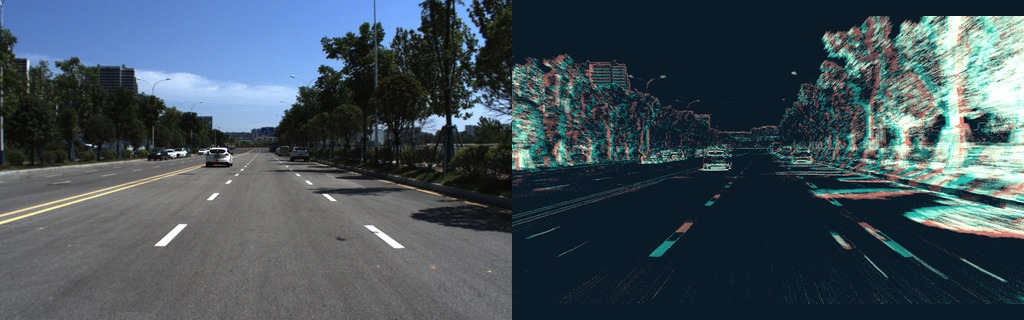
\includegraphics[width=\linewidth]{figures/evttc_ccrm_poster.jpg}
  \caption{\textbf{Real RGB and event observations from EvTTC.} Left: Blackfly left-camera frame 287 at $t=14.350374$\,s in recording \texttt{CCRm-low-0-overlap-0}. Right: Prophesee left-camera events in $[t-100\,\mathrm{ms},t)$, with positive counts in turquoise and negative counts in coral; overlap can appear pale. Counts use log scaling and an occupied-pixel 95th-percentile display scale. The RGB display swaps stored channels 0 and 2 to match the dataset publisher's visualization; the model-input crops preserve the runtime channel order. Images are resized for display and retain separate sensor coordinates. Source: EvTTC, Sun et al.\ \citep{evttc}; the same excerpt is used in the project website.}
  \label{fig:real-evttc-scene}
\end{figure}

The RGB view preserves scene appearance while event polarities reveal moving contours and contrast boundaries. The model receives localized object crops in a common coordinate frame across causal endpoints, preserving apparent scale change. Appendix~\ref{sec:real-inputs} shows the temporal crop triplets and twelve event input planes for this recording, with their timestamps and extraction provenance.


\subsection{Benchmark score decompositions}
\begin{figure}[htbp]
\centering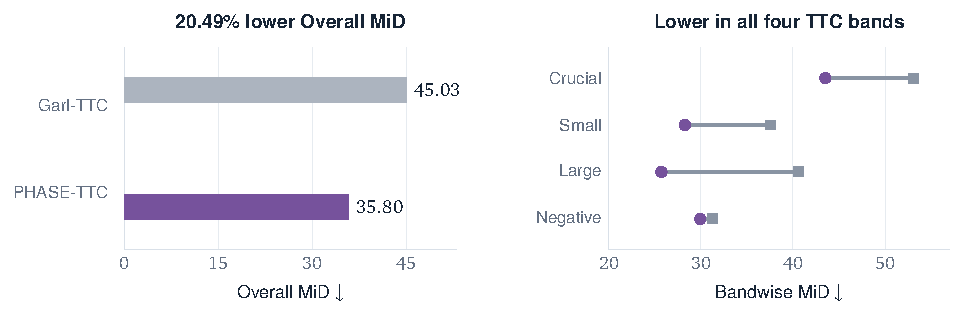
\includegraphics[width=\linewidth]{figures/rev_hero.pdf}
\caption{\textbf{Archived GarlTTC Test results, 28 October 2026.} Overall MiD and the four TTC bands compare the complete PHASE-TTC and Garl-TTC submissions. Both report 0\% scorer-defined failures across 6,762 tokens.}
\label{fig:official}
\end{figure}
\begin{figure}[H]
\centering
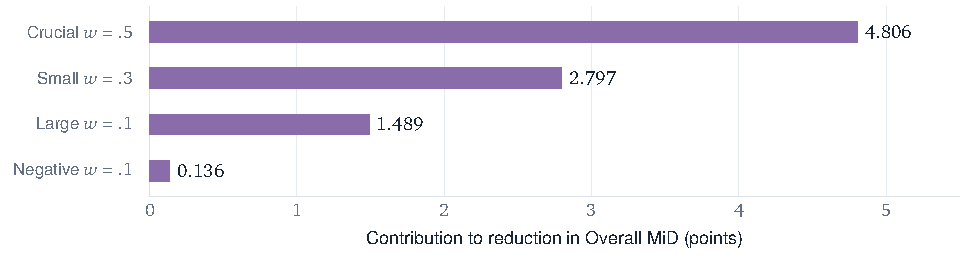
\includegraphics[width=.92\linewidth]{figures/rev_weighted.pdf}
\caption{\textbf{Bandwise contributions to the Overall MiD difference.} Crucial and small TTC account for about 82\% under the benchmark's $0.5/0.3/0.1/0.1$ weights. Table~\ref{tab:official-weighted-contributions} gives the rounding reconciliation. \evidence{B01,B02}}
\label{fig:official-weighted-contributions}
\end{figure}

\subsection{Transfer error distributions}
\begin{figure}[H]
\centering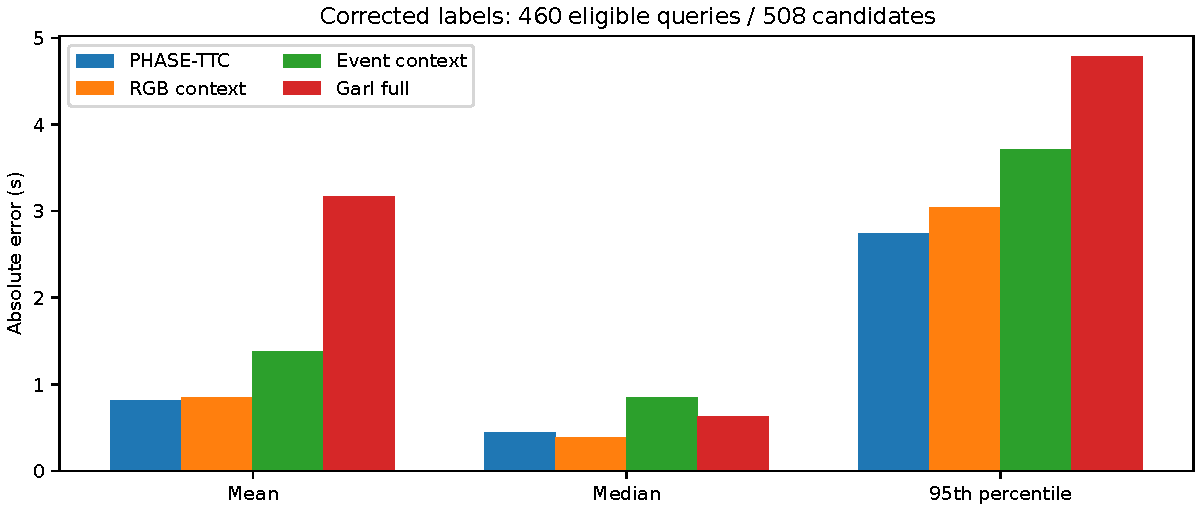
\includegraphics[width=.94\linewidth]{figures/audit_transfer_summary.pdf}
\caption{\textbf{Corrected frozen-transfer error summaries.} PHASE-TTC and RGB use the same \AuditTransferCount{} eligible queries after reassociating all 508 candidates. Lower point mean and p95 favor fusion; lower median favors RGB. Paired intervals are reported separately in Table~\ref{tab:audit-transfer-bootstrap}.}
\label{fig:transfer-tradeoff}
\end{figure}
\begin{figure}[htbp]
\centering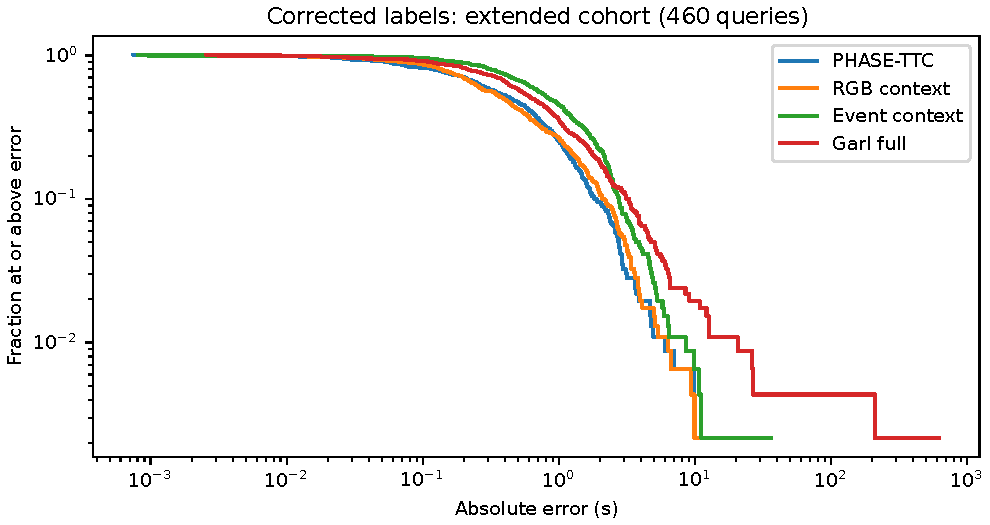
\includegraphics[width=\linewidth]{figures/audit_transfer_exceedance.pdf}
\caption{\textbf{Corrected absolute-error exceedance.} Curves include all \AuditTransferCount{} eligible transfer queries with equal query weights. No signed prediction is clipped and no extreme error is removed.}
\label{fig:transfer-exceedance}
\end{figure}
